\documentclass{article}

\usepackage{amsmath}
\usepackage{amssymb}

\usepackage{tikz}
\usetikzlibrary{calc}
\usetikzlibrary{external}
\tikzexternalize[prefix=idiagrams/]
\tikzset{every picture/.append style={scale=2}, every node/.style={transform shape}}

\begin{document}
% Measure macros
\newcommand{\op}[1] {\ensuremath{\operatorname{#1}}}
\renewcommand{\H}   {\op{H}}
\newcommand{\I}     {\op{I}}
\newcommand{\T}     {\op{T}}
\newcommand{\B}     {\op{B}}
\newcommand{\R}     {\op{R}}
\newcommand{\K}     {\op{K}}
\newcommand{\meet}  {\curlywedge}

% Definition of variables
\def \r {2cm}

\def \X {(-1, {-1/3*sqrt(3)}) circle (\r)}
\def \Y {( 1, {-1/3*sqrt(3)}) circle (\r)}
\def \Z {( 0, { 2/3*sqrt(3)}) circle (\r)}

\def \Ktwo   {(0, {-1/3*sqrt(3)}) circle (2/5*\r)}
\def \Kthree {(0, 0)              circle (1/3*\r)}

\colorlet{X color}{black}
\colorlet{Y color}{black}
\colorlet{Z color}{black}

% draw the I-diagram outlines
\newcommand{\drawIDtwo} {
    \draw [ultra thick, X color] \X;
    \draw [ultra thick, Y color] \Y;
}
\newcommand{\labelIDtwo}[2] {
    \draw (-2.5, 1.5) node [scale=1.5] {#1};
    \draw ( 2.5, 1.5) node [scale=1.5] {#2};
}
\newcommand{\drawIDthree} {
    \draw [ultra thick, X color] \X;
    \draw [ultra thick, Y color] \Y;
    \draw [ultra thick, Z color] \Z;
}
\newcommand{\labelIDthree}[3] {
    \draw (-2.75, -2.25) node [scale=1.5] {#1};
    \draw ( 2.75, -2.25) node [scale=1.5] {#2};
    \draw ( 2.00,  2.75) node [scale=1.5] {#3};
}

% fills for the 2-variable I-diagram
\newcommand{\IXGY}[1] {
    \begin{scope}[even odd rule]
        \clip \Y \X;
        \fill [black, fill opacity=#1] \X;
    \end{scope}
}
\newcommand{\IYGX}[1] {
    \begin{scope}[even odd rule]
        \clip \X \Y;
        \fill [black, fill opacity=#1] \Y;
    \end{scope}
}
\newcommand{\IXY}[1] {
    \begin{scope}[even odd rule]
        \clip \X;
        \fill [black, fill opacity=#1] \Y;
    \end{scope}
}
\newcommand{\fillIDtwo}[2] {
    \IXGY{#1}
    \IYGX{#1}
    \IXY{#2}
}

% fills for the 3-variable I-diagram
\newcommand{\IXGYZ}[1] {
    \begin{scope}[even odd rule]
        \clip \Y \X;
        \clip \Z \X;
        \fill [black, fill opacity=#1] \X;
    \end{scope}
}
\newcommand{\IYGXZ}[1] {
    \begin{scope}[even odd rule]
        \clip \X \Y;
        \clip \Z \Y;
        \fill [black, fill opacity=#1] \Y;
    \end{scope}
}
\newcommand{\IZGXY}[1] {
    \begin{scope}[even odd rule]
        \clip \X \Z;
        \clip \Y \Z;
        \fill [black, fill opacity=#1] \Z;
    \end{scope}
}
\newcommand{\IXYGZ}[1] {
    \begin{scope}[even odd rule]
        \clip \Z \X;
        \clip \X;
        \fill [black, fill opacity=#1] \Y;
    \end{scope}
}
\newcommand{\IXZGY}[1] {
    \begin{scope}[even odd rule]
        \clip \Y \X;
        \clip \X;
        \fill [black, fill opacity=#1] \Z;
    \end{scope}
}
\newcommand{\IYZGX}[1] {
    \begin{scope}[even odd rule]
        \clip \X \Y;
        \clip \Y;
        \fill [black, fill opacity=#1] \Z;
    \end{scope}
}
\newcommand{\IXYZ}[1] {
    \begin{scope}[even odd rule]
        \clip \X;
        \clip \Y;
        \fill [black, fill opacity=#1] \Z;
    \end{scope}
}
\newcommand{\fillIDthree}[3] {
    \IXGYZ{#1}
    \IYGXZ{#1}
    \IZGXY{#1}
    \IXYGZ{#2}
    \IXZGY{#2}
    \IYZGX{#2}
    \IXYZ{#3}
}

\setlength{\parskip}{5mm}

%%% Measures

%% Shannon

\tikzsetnextfilename{h_x}
\begin{tikzpicture}
    \drawIDtwo
    \labelIDtwo{$X_0$}{$X_1$}
    \fill [black, fill opacity=0.25] \X;
    \node[anchor=south, scale=1.5] at (current bounding box.north) {$\H[X_0]$};
\end{tikzpicture}

\tikzsetnextfilename{h_y}
\begin{tikzpicture}
    \drawIDtwo
    \labelIDtwo{$X_0$}{$X_1$}
    \fill [black, fill opacity=0.25] \Y;
    \node[anchor=south, scale=1.5] at (current bounding box.north) {$\H[X_1]$};
\end{tikzpicture}

\tikzsetnextfilename{h_xgy}
\begin{tikzpicture}
    \drawIDtwo
    \labelIDtwo{$X_0$}{$X_1$}
    \begin{scope}[even odd rule]
        \clip \X \Y;
        \fill [black, fill opacity=0.25] \X;
    \end{scope}
    \node[anchor=south, scale=1.5] at (current bounding box.north) {$\H[X_0|X_1]$};
\end{tikzpicture}

\tikzsetnextfilename{h_ygx}
\begin{tikzpicture}
    \drawIDtwo
    \labelIDtwo{$X_0$}{$X_1$}
    \begin{scope}[even odd rule]
        \clip \Y \X;
        \fill [black, fill opacity=0.25] \Y;
    \end{scope}
    \node[anchor=south, scale=1.5] at (current bounding box.north) {$\H[X_1|X_0]$};
\end{tikzpicture}

%% Entropy

\tikzsetnextfilename{h_xy}
\begin{tikzpicture}
    \drawIDtwo
    \labelIDtwo{$X_0$}{$X_1$}
    \fillIDtwo{0.25}{0.25}
    \node[anchor=south, scale=1.5] at (current bounding box.north) {$\H[X_0, X_1]$};
\end{tikzpicture}

\tikzsetnextfilename{h_xyz}
\begin{tikzpicture}
    \drawIDthree
    \labelIDthree{$X_0$}{$X_1$}{$X_2$}
    \fillIDthree{0.25}{0.25}{0.25}
    \node[anchor=south, scale=1.5] at (current bounding box.north) {$\H[X_0, X_1, X_2]$};
\end{tikzpicture}

%% Co-Information

\tikzsetnextfilename{i_xy}
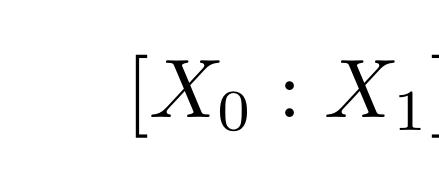
\begin{tikzpicture}
    \drawIDtwo
    \labelIDtwo{$X_0$}{$X_1$}
    \fillIDtwo{0.0}{0.25}
    \node[anchor=south, scale=1.5] at (current bounding box.north) {$\I[X_0 : X_1]$};
\end{tikzpicture}

\tikzsetnextfilename{i_xyz}
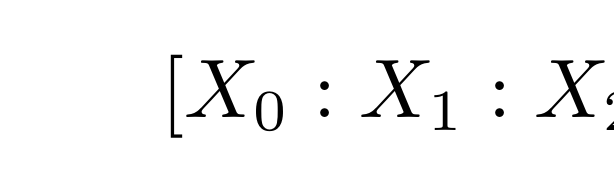
\begin{tikzpicture}
    \drawIDthree
    \labelIDthree{$X_0$}{$X_1$}{$X_2$}
    \fillIDthree{0.0}{0.0}{0.25}
    \node[anchor=south, scale=1.5] at (current bounding box.north) {$\I[X_0 : X_1 : X_2]$};
\end{tikzpicture}

%% Total Correlation

\tikzsetnextfilename{t_xy}
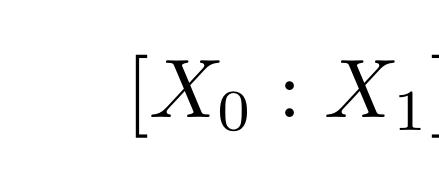
\begin{tikzpicture}
    \drawIDtwo
    \labelIDtwo{$X_0$}{$X_1$}
    \fillIDtwo{0.0}{0.25}
    \node[anchor=south, scale=1.5] at (current bounding box.north) {$\T[X_0 : X_1]$};
\end{tikzpicture}

\tikzsetnextfilename{t_xyz}
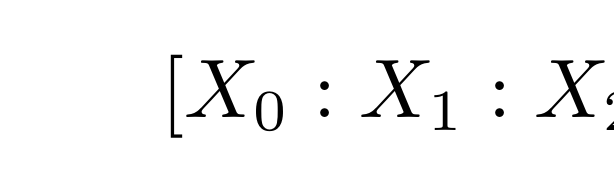
\begin{tikzpicture}
    \drawIDthree
    \labelIDthree{$X_0$}{$X_1$}{$X_2$}
    \fillIDthree{0.0}{0.25}{0.5}
    \node[anchor=south, scale=1.5] at (current bounding box.north) {$\T[X_0 : X_1 : X_2]$};
\end{tikzpicture}

%% Binding Information

\tikzsetnextfilename{b_xy}
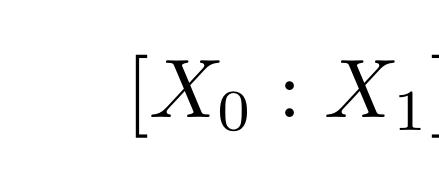
\begin{tikzpicture}
    \drawIDtwo
    \labelIDtwo{$X_0$}{$X_1$}
    \fillIDtwo{0.0}{0.25}
    \node[anchor=south, scale=1.5] at (current bounding box.north) {$\B[X_0 : X_1]$};
\end{tikzpicture}

\tikzsetnextfilename{b_xyz}
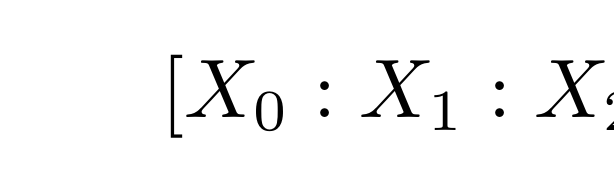
\begin{tikzpicture}
    \drawIDthree
    \labelIDthree{$X_0$}{$X_1$}{$X_2$}
    \fillIDthree{0.0}{0.25}{0.25}
    \node[anchor=south, scale=1.5] at (current bounding box.north) {$\B[X_0 : X_1 : X_2]$};
\end{tikzpicture}

%% Residual Entropy

\tikzsetnextfilename{r_xy}
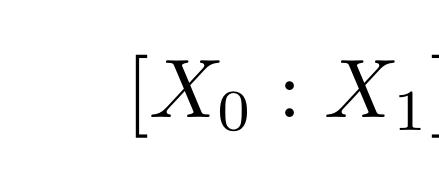
\begin{tikzpicture}
    \drawIDtwo
    \labelIDtwo{$X_0$}{$X_1$}
    \fillIDtwo{0.25}{0.0}
    \node[anchor=south, scale=1.5] at (current bounding box.north) {$\R[X_0 : X_1]$};
\end{tikzpicture}

\tikzsetnextfilename{r_xyz}
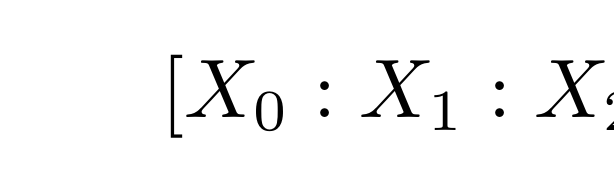
\begin{tikzpicture}
    \drawIDthree
    \labelIDthree{$X_0$}{$X_1$}{$X_2$}
    \fillIDthree{0.25}{0.0}{0.0}
    \node[anchor=south, scale=1.5] at (current bounding box.north) {$\R[X_0 : X_1 : X_2]$};
\end{tikzpicture}

%% Gács-Körner Common Information

\tikzsetnextfilename{k_xy}
\begin{tikzpicture}
    \drawIDtwo
    \labelIDtwo{$X_0$}{$X_1$}
    \draw [ultra thick] \Ktwo;
    \fill [black, fill opacity=0.25] \Ktwo;
    \node[anchor=south, scale=1.5] at (current bounding box.north) {$\K[X_0 : X_1]$};
\end{tikzpicture}

\tikzsetnextfilename{k_xyz}
\begin{tikzpicture}
    \drawIDthree
    \labelIDthree{$X_0$}{$X_1$}{$X_2$}
    \draw [ultra thick] \Kthree;
    \fill [black, fill opacity=0.25] \Kthree;
    \node[anchor=south, scale=1.5] at (current bounding box.north) {$\K[X_0 : X_1 : X_2]$};
\end{tikzpicture}

\tikzsetnextfilename{red_xy}
\begin{tikzpicture}
    \drawIDthree
    \labelIDthree{$X_0$}{$X_1$}{$Y$}
    \draw [ultra thick] \Ktwo;
    \begin{scope}[even odd rule]
        \clip \Z;
        \fill [black, fill opacity=0.25] \Ktwo;
    \end{scope}
    \node[anchor=south, scale=1.5] at (current bounding box.north) {$\I[X_0 \meet X_1 : Y]$};
\end{tikzpicture}

\end{document}
